\section{Admin}
The Admin Portal was built for documenting the locations of iBeacons as well as any other pertinent information. The overall
structure was based on the LAMP (Linux, Apache web server, MySQL, and PHP) model. The user of the portal has the ability to add beacon data, edit beacon data,
delete beacon data, view the beacon data, and geo calibrate the location service. The Geo Calibrate feature allowed for the
user to drag a shape over the building that the BLE location system will be implemented in. See Appendix A for screenshots of some of these features. The anchor points in latitude
and longitude were tracked and then used to calculate a ratio that can be used by the system to convert abstract units to
real world latitude and longitude. The home page can be seen in figure ***.

\begin{figure}[h]
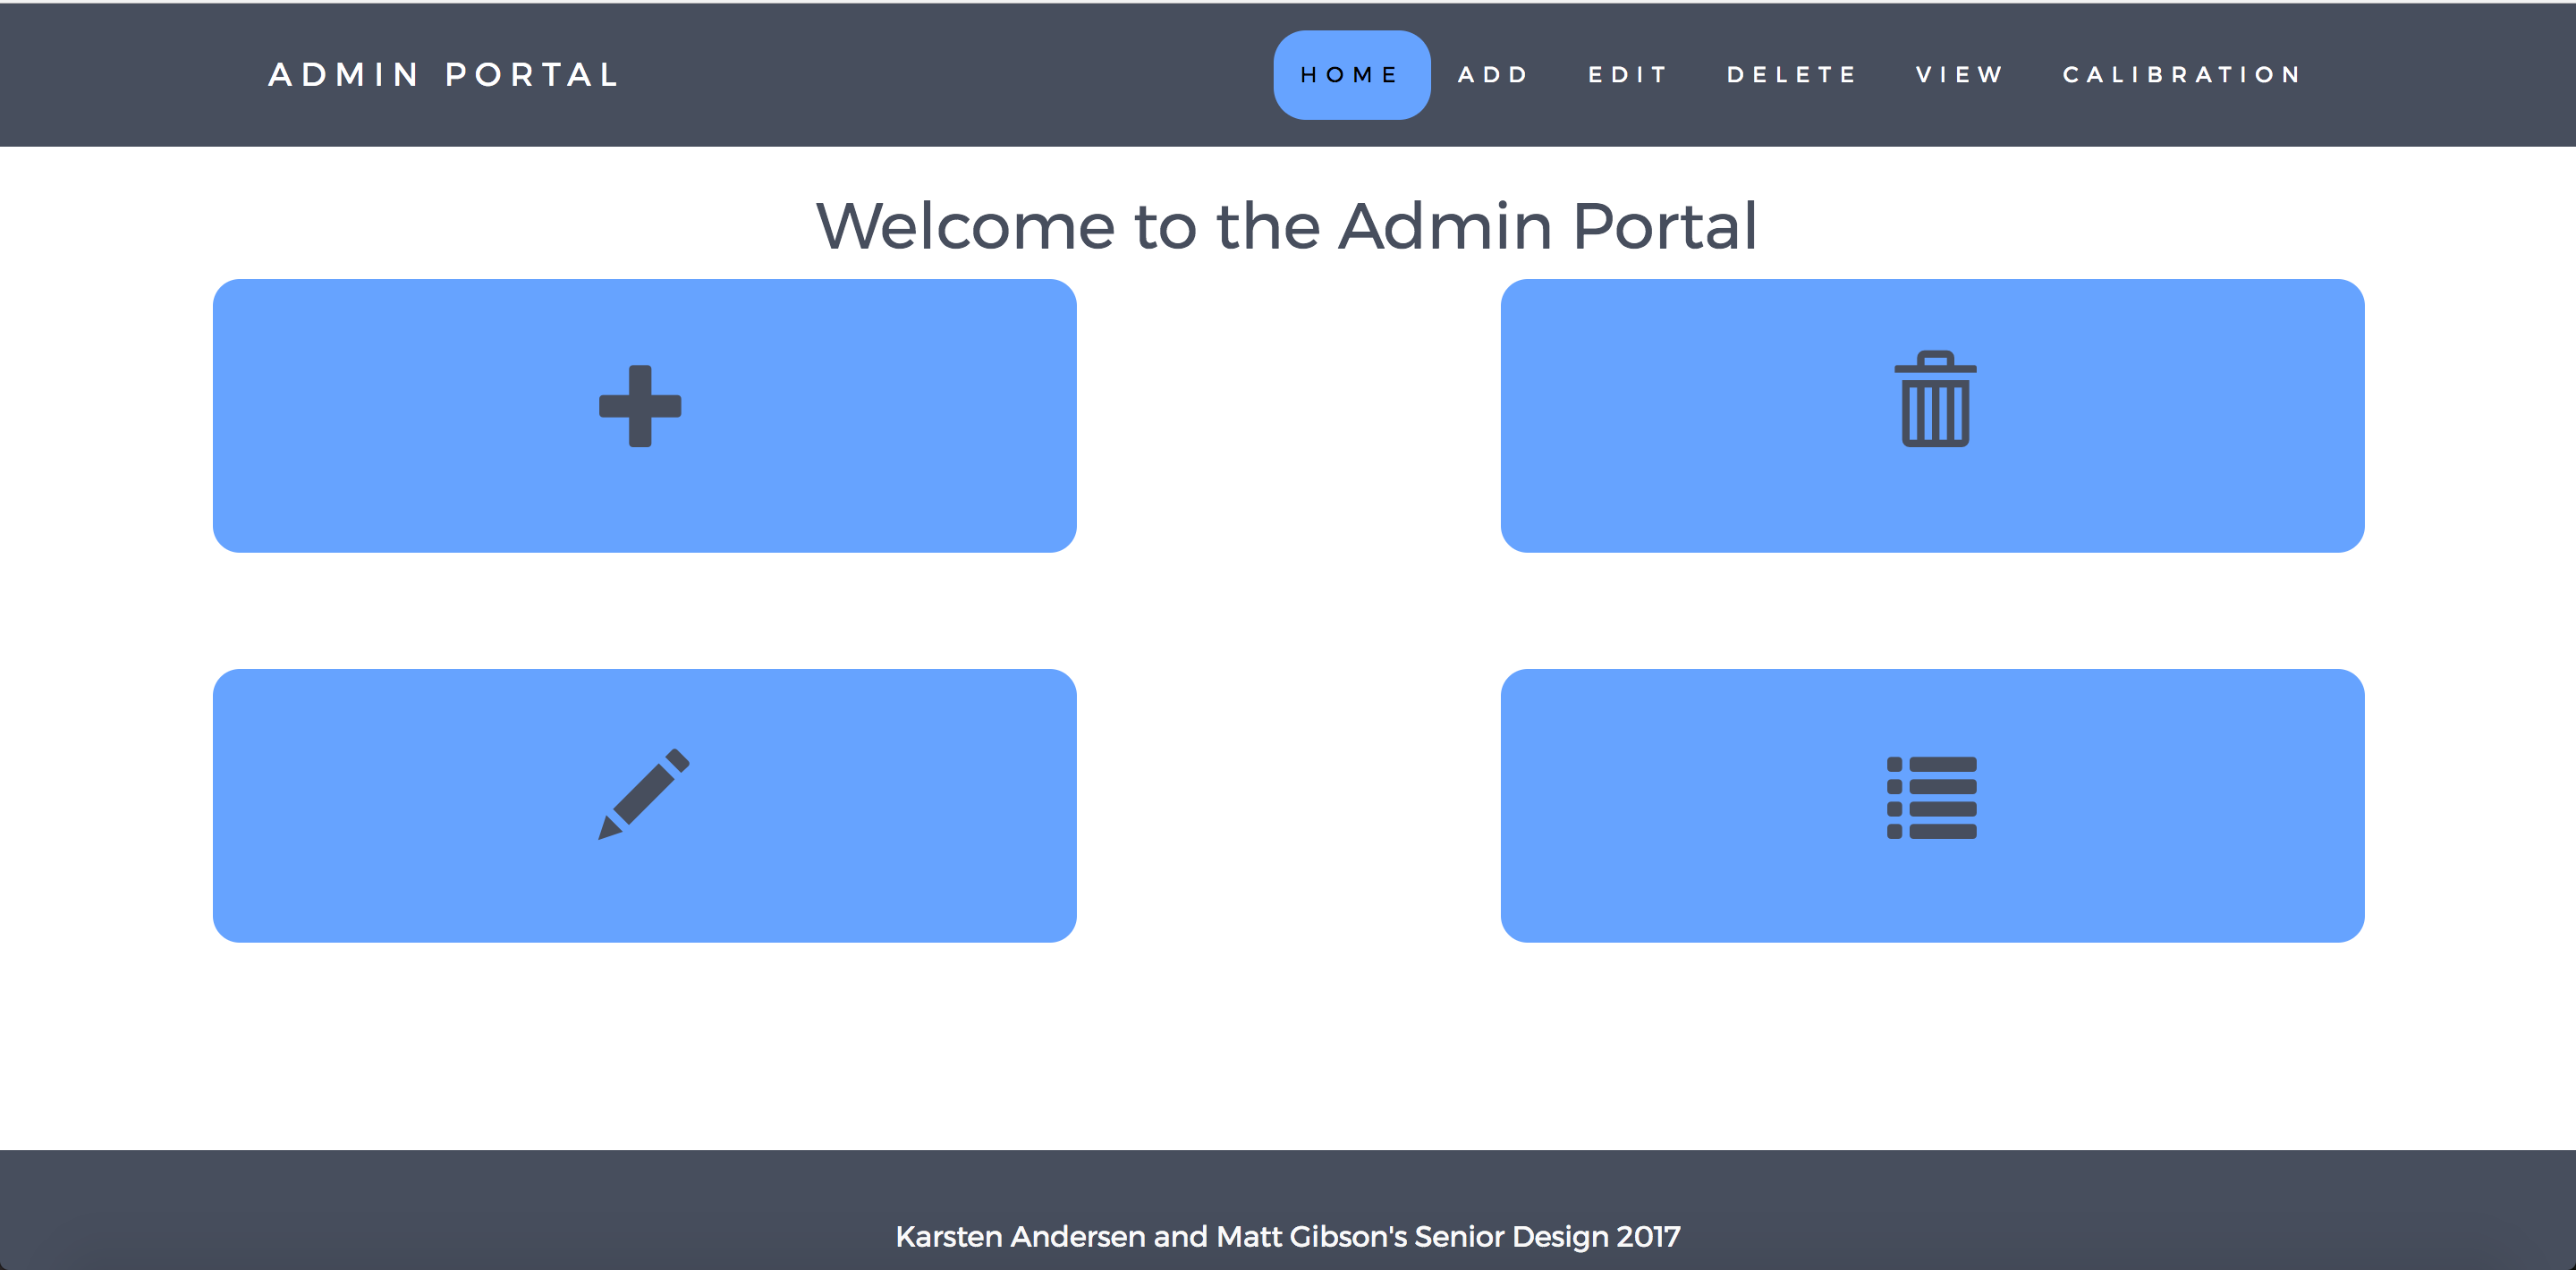
\includegraphics[width=1\textwidth]{images/homeAdmin.png}
\caption{Home Page of Admin Portal}
\end{figure}

\subsection{Front End}
The front end was built upon the traditional web programming languages. HTML5 was used for the basic skeleton of the website
and CSS3 was used for the aesthetics. Javascript was used for the front end functionality and jQuery was used to make the AJAX calls
and to simplify the DOM manipulation. Bootstrap was used to give the site a mobile responsive design to allow the user to have the ability
to enter and manipulate beacon data on the go with a smaller device. Finally the Google Maps API was used to allow the system to obtain
real world latitude and longitude values.

\subsection{Back End}
Since the overall structure was based on the LAMP model, the website was hosted on an Apache Web Server with an HTTPS connection. The admin portal can be
found at andersenkarsten.com/seniorDesign. The PHP programming language was used as the intermediary between the front end and the MySQL database.
The MySQL database was used to store the important information for the iBeacons within two tables. The first table contained information having to do with beacon identification as well as location including:
name, UUID, minor value, major value, and XYZ coordinates. The second table contained the four anchor points of the latitude and longitude, the ratio data for the abstract to real world calculation, and the unique identifier for that layout.
The data supplied to and from the PHP and MySQL were done through queries and transported to the front end through JSON.
